%!TEX program = xelatex

\documentclass{progartcn}
\usepackage{graphicx}
\usepackage[dvipsnames]{xcolor}
\usepackage{wrapfig}
\usepackage{enumerate}
\usepackage{amsmath,mathrsfs,amsfonts}
\usepackage{booktabs}
\usepackage{tabularx}
\usepackage{colortbl}
\usepackage{multirow,makecell}
\usepackage{multicol}
\usepackage{ulem} % \uline
\usepackage{listings}
\usepackage{tikz}
\usepackage{tcolorbox}
\usepackage{fontawesome}


\title{\bfseries\sffamily
  计算机系统结构实验1 \\ FPGA基础实验:LED Flow Water Light
}
\author{胡晨志 521021910107}
\date{}


\begin{document}

\sloppy % 解决中英文混排文字超出边界问题


\maketitle
\thispagestyle{empty}

\begin{abstract}
\noindent 在lab01中,我学习了Verilog语言并实现了flowing light功能,对Verilog的基本语法有了大致的了解,并对Vivado的编程环境、项目流程、调试方合仿真手段有了基本的了解。

\vspace{2ex}
\noindent \textbf{关键字:}Vivado,\hspace{.5em}Verilog
\end{abstract}

\tableofcontents

\setcounter{page}{0}
\newpage

\section{实验目的}

\begin{itemize}
  \item 掌握 Xilinx 逻辑设计工具 Vivado 的基本操作
  \item 掌握使用 Verilog HDL 进行简单的逻辑设计
  \item 掌握仿真功能
  \item 使用 1/0 Planing 添加管脚约束
  \item 生成 Bitstream 文件
  \item 上板验证
\end{itemize}

\section{原理分析}

\subsection{Vivado 工程的基本组成}

Vivado 工程的基本组成如下:

\begin{itemize}
  \item design source .v 文件
  \item simulation source .v 文件
  \item constrain .xdc 文件(上板验证所需的管脚约束文件)
\end{itemize}

在本次实验中,对应的文件依次为 flowing\_light.v 文件、flowing\_light\_tb.v 文件和 lab01\_xdc.xdc 文件。

\subsection{flowing light原理}

Flowing light 要求在一定时间内8个LED等依次亮灭,最后一个 LED 灯熄灭,第一个 LED 灯循环亮起。在实现代码中,用时钟周期的上升沿来同步灯的亮灭,代码如</>CODE \ref{cd:1}所示。由代码克制控制 LED 的 \verb|light_reg| 每过384个时钟周期进行一次位移。

\begin{lstlisting}[language=verilog,caption={flowing light实现},label={cd:1}]
  always @ (posedge clock)
  begin
      if (reset)
          light_reg <= 8'h01;
      else if (cnt_reg == 24'h0ffffff)
          begin
              if (light_reg == 8'h80)
                  light_reg <= 8'h01;
              else
                  light_reg <= light_reg << 1;
          end
  end
\end{lstlisting}

\section{功能实现}

基于上述即可完成 flowing light 的功能。完整代码如</>CODE \ref{cd:2}所示。

\begin{lstlisting}[language=verilog,caption={flowing\_light.v},label={cd:2}]
  `timescale 1ns / 1ps 
  
  module flowing_light(
      input clock,
      input reset,
      output [7:0] led
      );
      reg [23 : 0] cnt_reg;
      reg [7 : 0] light_reg;
      always @ (posedge clock)
          begin
              if (reset)
                  cnt_reg <= 0;
              else
                  cnt_reg <= cnt_reg + 1;
          end
      always @ (posedge clock)
          begin
              if (reset)
                  light_reg <= 8'h01;
              else if (cnt_reg == 24'h0ffffff)
                  begin
                      if (light_reg == 8'h80)
                          light_reg <= 8'h01;
                      else
                          light_reg <= light_reg << 1;
                  end
          end
      assign led = light_reg;
  endmodule
\end{lstlisting}

实现 flowing\_light.v 后,生成 flowing\_light\_tb.v 的激励文件用以仿真测试,生成 lab01\_xdc.xdc 的管脚约束用以练习。

\section{结果验证}

\subsection{测试用激励文件}

按照实验指导书的要求编写 flowing\_light\_tb.v 文件,代码如</>CODE \ref{cd:3} 所示。

\begin{lstlisting}[language=verilog,caption={flowing\_light\_tb.v},label={cd:2}]
  `timescale 1ns / 1ps

  module flowing_light_tb(
  
      );
      reg clock;
      reg reset;
      wire [7 : 0] led;
      
      flowing_light u0(
          .clock(clock),
          .reset(reset),
          .led(led));
      
      parameter PERIOD = 10;
      
      always #(PERIOD*2) clock = !clock;
      
      initial begin
          clock = 1'b0;
          reset = 1'b0;
          #(PERIOD*2) reset = 1'b1;
          #(PERIOD*4) reset = 1'b0;
          
          //#580; reset = 1'b1;
      end
  endmodule
\end{lstlisting}

\subsection{reset 与基本逻辑的测试}

获得的仿真结果如图\ref{fig:1}所示。从图中可以看到 \verb|reset|,\verb|cnt_reg|,\verb|light_reg| 功能正常。

\begin{figure}[htbp]
  %是可选项 h表示的是here在这里插入,t表示的是在页面的顶部插入
  \centering
  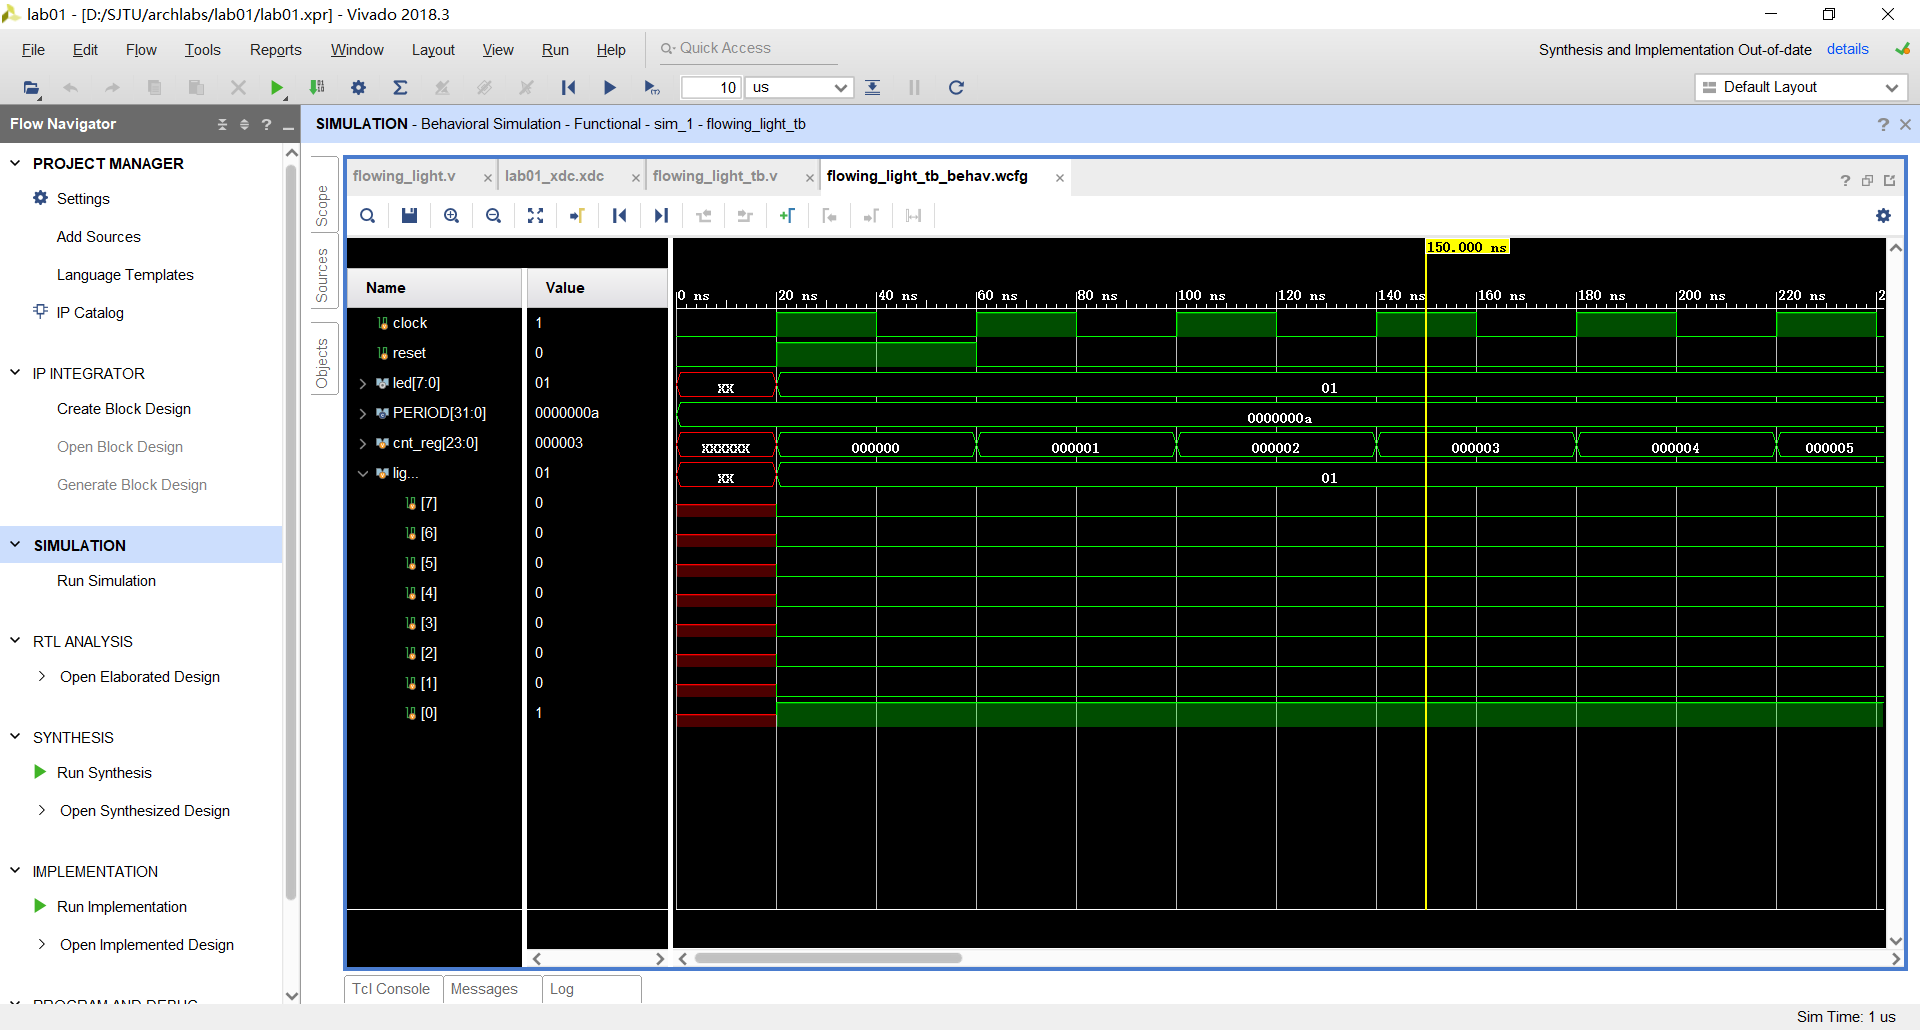
\includegraphics[scale=0.3]{../figure/01/lab01-1.PNG}
  \caption{实验结果1}\label{fig:1}
\end{figure}

\subsection{调整控制逻辑以观察位移}

上述仿真运行周期不够,计数器并没加到24位全是1波形显示已结束。将 \verb|cnt_reg| 改为两位后可观察到位移,代码如</>CODE \ref{cd:3} 所示,仿真结果如图 \ref{fig:2} 所示。

\begin{lstlisting}[language=verilog,caption={修改后的flowing light},label={cd:3}]
  reg [1 : 0] cnt_reg;
  reg [7 : 0] light_reg;
  always @ (posedge clock)
      begin
          if (reset)
              cnt_reg <= 0;
          else
              cnt_reg <= cnt_reg + 1;
      end
  always @ (posedge clock)
      begin
          if (reset)
              light_reg <= 8'h01;
          else if (cnt_reg == 2'b11)
              begin
                  if (light_reg == 8'h80)
                      light_reg <= 8'h01;
                  else
                      light_reg <= light_reg << 1;
              end
      end
  assign led = light_reg;
\end{lstlisting}

\begin{figure}[htbp]
  %是可选项 h表示的是here在这里插入,t表示的是在页面的顶部插入
  \centering
  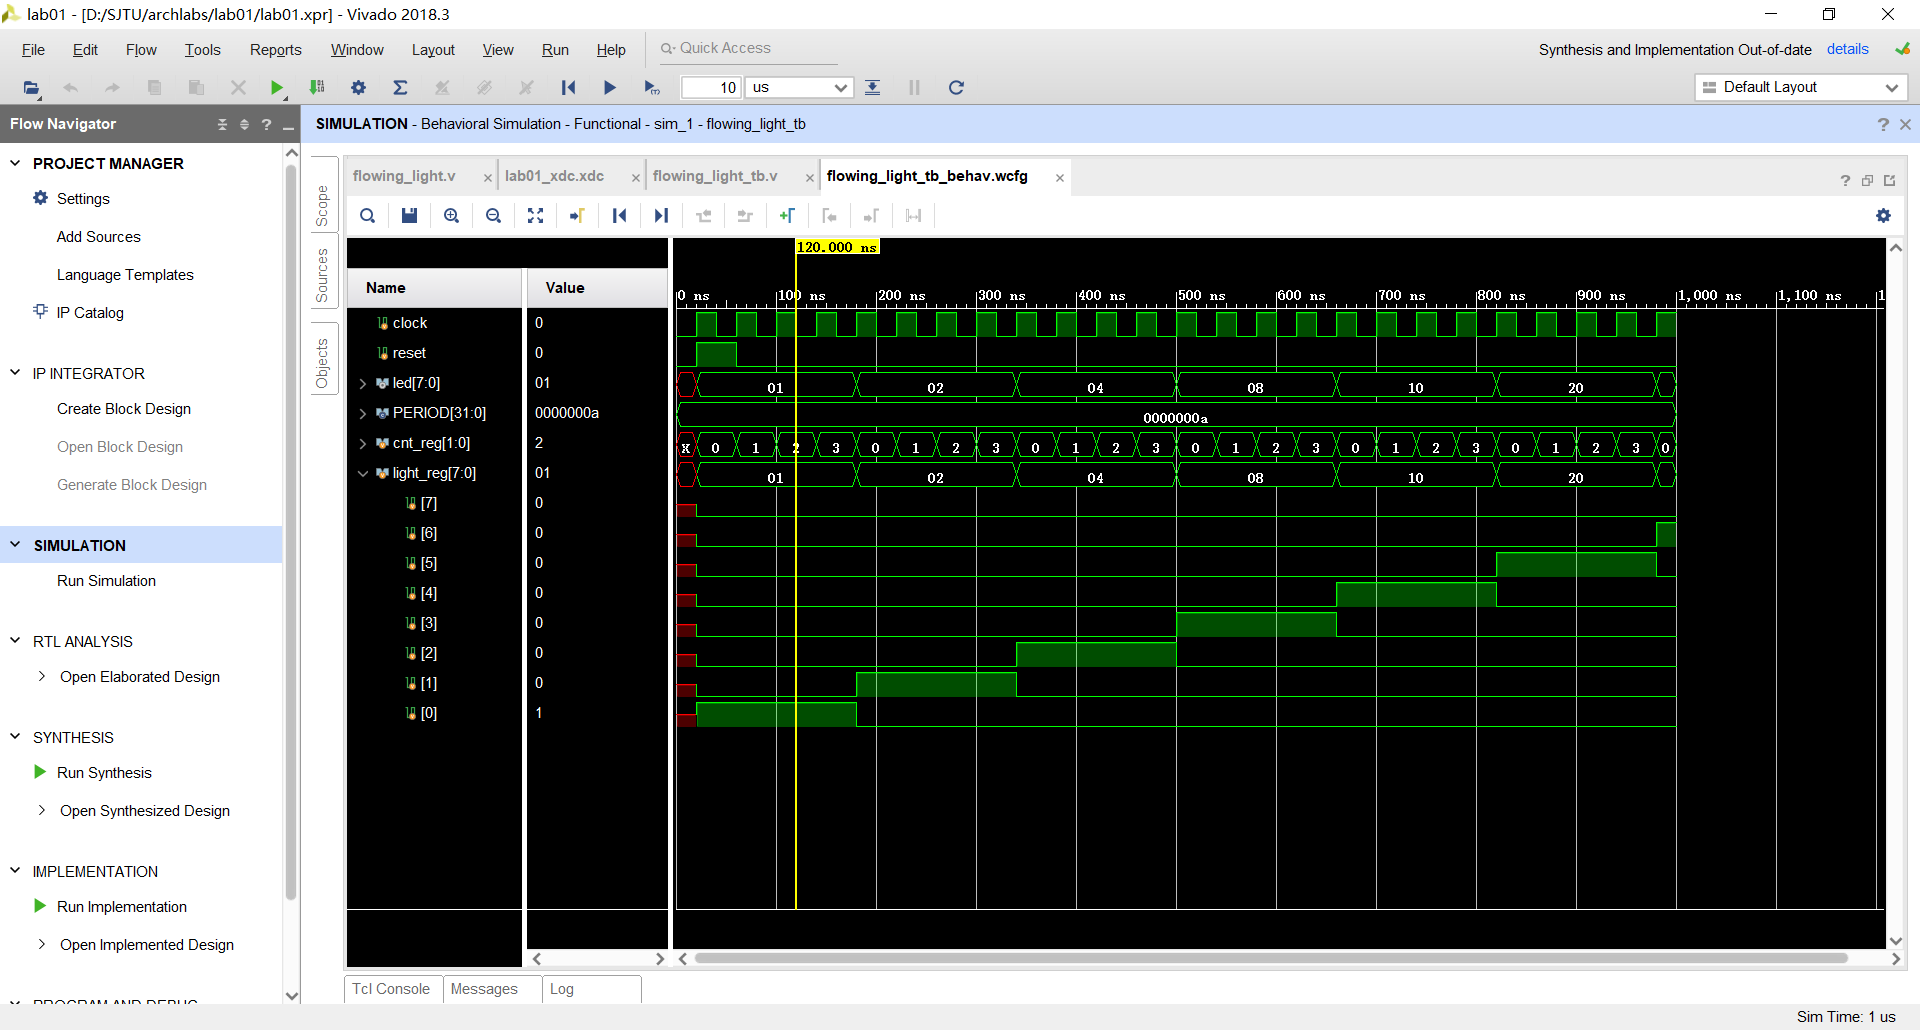
\includegraphics[scale=0.3]{../figure/01/lab01-2.PNG}
  \caption{实验结果2}\label{fig:2}
\end{figure}

\section{管脚约束}

管脚约束文件为 lab01\_xdc.xdc,代码如 </>CODE \ref{cd:4} 所示。在上板前,需要将 flowing\_light.v 文件也进行修改,代码如 </>CODE \ref{cd:5} 所示。

\begin{lstlisting}[caption={lab01\_xdc.xdc},label={cd:4}]
  set_property PACKAGE_PIN W23 [get_ports {led[7]}]
  set_property PACKAGE_PIN AB26 [get_ports {led[6]}]
  set_property PACKAGE_PIN Y25 [get_ports {led[5]}]
  set_property PACKAGE_PIN AA23 [get_ports {led[4]}]
  set_property PACKAGE_PIN Y23 [get_ports {led[3]}]
  set_property PACKAGE_PIN Y22 [get_ports {led[2]}]
  set_property PACKAGE_PIN AE21 [get_ports {led[1]}]
  set_property PACKAGE_PIN AF24 [get_ports {led[0]}]
  set_property PACKAGE_PIN AC18 [get_ports clock_p]
  set_property PACKAGE_PIN W13 [get_ports reset]
  set_property IOSTANDARD LVCMOS33 [get_ports {led[7]}]
  set_property IOSTANDARD LVCMOS33 [get_ports {led[6]}]
  set_property IOSTANDARD LVCMOS33 [get_ports {led[5]}]
  set_property IOSTANDARD LVCMOS33 [get_ports {led[4]}]
  set_property IOSTANDARD LVCMOS33 [get_ports {led[3]}]
  set_property IOSTANDARD LVCMOS33 [get_ports {led[2]}]
  set_property IOSTANDARD LVCMOS33 [get_ports {led[1]}]
  set_property IOSTANDARD LVCMOS33 [get_ports {led[0]}]
  set_property IOSTANDARD LVDS [get_ports clock_p]
  set_property IOSTANDARD LVCMOS18 [get_ports reset]
\end{lstlisting}

\begin{lstlisting}[language=verilog,caption={flowing\_light.v最终代码},label={cd:5}]
  `timescale 1ns / 1ps
  module flowing_light(
      input clock_p,
      input clock_n,
      input reset,
      output [7:0] led
      );
      reg [23 : 0] cnt_reg;
      reg [7 : 0] light_reg;
      
      IBUFGDS IBUFGDS_inst (
          .O(CLK_i),
          .I(clock_p),
          .IB(clock_n)
      );
      
      always @ (posedge CLK_i)
          begin
              if (!reset)
                  cnt_reg <= 0;
              else
                  cnt_reg <= cnt_reg + 1;
          end
      always @ (posedge CLK_i)
          begin
              if (!reset)
                  light_reg <= 8'h01;
              else if (cnt_reg == 24'h0ffffff)
                  begin
                      if (light_reg == 8'h80)
                          light_reg <= 8'h01;
                      else
                          light_reg <= light_reg << 1;
                  end
          end
      assign led = light_reg;
  endmodule
\end{lstlisting}

\section{总结与反思}

这是我第一次接触 Vivado 开发环境和 Verilog 语言,刚上手时闹了不少笑话,比如把代码写到 I/O 说明中。此外由于对工程流程不熟悉,Lab01花了我大量的时间。好在经过一个上午的摸索之后我还是成功地完成了本次实验,受益匪浅。感谢老师和助教的指导!

\end{document}
